% WT-HALI Research Presentation
% Author: Dhruv Joshi
% Redesigned: Explanatory style with motivated design choices

\documentclass[aspectratio=169,12pt]{beamer}
\usetheme{Berkeley}
\usecolortheme{seahorse}

% Packages
\usepackage{tikz}
\usepackage{pgfplots}
\usepackage{booktabs}
\usepackage{multirow}
\usepackage{algorithm}
\usepackage{algorithmic}
\usepackage{amsmath}
\usepackage{amssymb}
\usepackage{graphicx}
\usepackage{listings}
\usepackage{xcolor}

\usetikzlibrary{shapes,arrows,positioning,fit,backgrounds,calc}
\pgfplotsset{compat=1.17}

% Title Information
\title[WT-HALI]{WT-HALI: Write-Through Hierarchical Adaptive Learned Index}
\subtitle{Combining Learned Efficiency with Traditional Robustness}
\author[D. Joshi]{Dhruv Joshi\\ \texttt{jdhruv1503@gmail.com}}
\institute{Operating Systems Course Project}
\date{\today}

% Custom colors
\definecolor{codegreen}{rgb}{0,0.6,0}
\definecolor{codegray}{rgb}{0.5,0.5,0.5}
\definecolor{codepurple}{rgb}{0.58,0.0.82}
\definecolor{backcolour}{rgb}{0.95,0.95,0.92}

\lstdefinestyle{mystyle}{
    backgroundcolor=\color{backcolour},
    commentstyle=\color{codegreen},
    keywordstyle=\color{blue},
    numberstyle=\tiny\color{codegray},
    stringstyle=\color{codepurple},
    basicstyle=\ttfamily\footnotesize,
    breakatwhitespace=false,
    breaklines=true,
    captionpos=b,
    keepspaces=true,
    numbers=left,
    numbersep=5pt,
    showspaces=false,
    showstringspaces=false,
    showtabs=false,
    tabsize=2
}
\lstset{style=mystyle}

\begin{document}

% ============================================================
% TITLE SLIDE
% ============================================================
\begin{frame}
\titlepage
\end{frame}

% ============================================================
% OUTLINE
% ============================================================
\begin{frame}{Outline}
\tableofcontents
\end{frame}

% ============================================================
% SECTION 1: THE PROBLEM
% ============================================================
\section{The Problem: Learned Indexes Can't Handle Writes}

\begin{frame}{The Learned Index Promise}

\begin{block}{The Big Idea (Kraska et al., SIGMOD 2018)}
Replace pointer-chasing B+Trees with machine learning models
\end{block}

\pause

\textbf{Why?} Imagine you're looking for a book in a library...

\pause

\begin{columns}
\column{0.5\textwidth}
\textbf{Traditional Index (B+Tree):}
\begin{itemize}
    \item Follow pointers room → shelf → book
    \item \textcolor{red}{$\sim$12 cache misses per lookup}
    \item But: Works for any data
\end{itemize}

\pause

\column{0.5\textwidth}
\textbf{Learned Index:}
\begin{itemize}
    \item Memorize the pattern: "Book X is at position Y"
    \item \textcolor{green}{$\sim$2-3 cache misses}
    \item But: What if books move?
\end{itemize}
\end{columns}

\end{frame}

\begin{frame}{Concrete Example: Looking Up Key 12345}

\textbf{Scenario:} 1 million sorted integers

\pause

\vspace{0.3cm}

\textbf{B+Tree approach:}
\begin{enumerate}
    \item Check root node → pointer to internal node (cache miss)
    \pause
    \item Check internal node → pointer to leaf (cache miss)
    \pause
    \item Check leaf node → find key (cache miss)
    \pause
    \item Total: \textcolor{red}{3+ cache misses, $\sim$20-30 ns}
\end{enumerate}

\pause

\vspace{0.3cm}

\textbf{Learned Index (RMI) approach:}
\begin{enumerate}
    \item Model predicts: "Key 12345 is at position $\approx$ 500,234"
    \pause
    \item Binary search $\pm$64 positions around prediction
    \pause
    \item Total: \textcolor{green}{1-2 cache misses, $\sim$70-90 ns}
\end{enumerate}

\pause

\vspace{0.3cm}

\textbf{Wait... that's SLOWER!} \pause $\rightarrow$ But uses \textcolor{green}{16 bytes/key vs B+Tree's 50+ bytes/key}

\end{frame}

\begin{frame}{The Catch: Dynamic Updates}

\textbf{Problem:} What happens when you insert a new key?

\pause

\vspace{0.3cm}

\textbf{Example:} Insert key 12340 into our learned index

\pause

\begin{center}
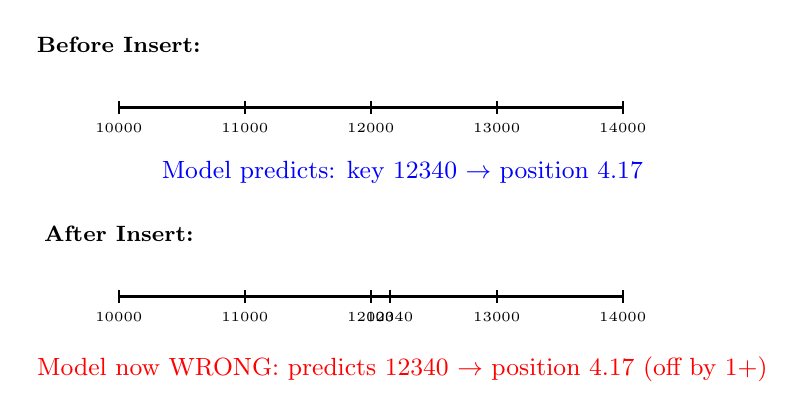
\begin{tikzpicture}[scale=0.8]
% Before
\node[font=\footnotesize\bfseries] at (0,3) {Before Insert:};
\draw[thick] (0,2) -- (8,2);
\foreach \x/\key in {0/10000, 2/11000, 4/12000, 6/13000, 8/14000} {
    \draw[thick] (\x,1.9) -- (\x,2.1);
    \node[below, font=\tiny] at (\x,1.9) {\key};
}
\node[below, color=blue, font=\small] at (4.5,1.3) {Model predicts: key 12340 $\rightarrow$ position 4.17};

\pause

% After
\node[font=\footnotesize\bfseries] at (0,0) {After Insert:};
\draw[thick] (0,-1) -- (8,-1);
\foreach \x/\key in {0/10000, 2/11000, 4/12000, 4.3/12340, 6/13000, 8/14000} {
    \draw[thick] (\x,-1.1) -- (\x,-0.9);
    \node[below, font=\tiny] at (\x,-1.1) {\key};
}

\pause

\node[below, color=red, font=\small] at (4.5,-1.8) {Model now WRONG: predicts 12340 $\rightarrow$ position 4.17 (off by 1+)};

\end{tikzpicture}
\end{center}

\pause

\vspace{0.2cm}

\textbf{Solution?} Retrain the model... but that takes \textcolor{red}{milliseconds to seconds!}

\pause

\textbf{Result:} Pure learned indexes get $\sim$100K inserts/sec vs B+Tree's $\sim$20M inserts/sec

\end{frame}

\begin{frame}{Motivation: We Need BOTH}

\begin{center}
\large
\textbf{Can we get the memory efficiency of learned indexes}\\
\textbf{AND the write performance of traditional structures?}
\end{center}

\pause

\vspace{0.5cm}

\begin{columns}
\column{0.5\textwidth}
\textbf{What We Want:}
\begin{itemize}
    \item<2-> Fast lookups (< 100 ns)
    \item<3-> High insert throughput (> 10M ops/sec)
    \item<4-> Low memory (< 20 bytes/key)
    \item<5-> 100\% correctness
\end{itemize}

\column{0.5\textwidth}
\textbf{Existing Solutions Fall Short:}
\begin{itemize}
    \item<2-> B+Tree: Fast writes, high memory
    \item<3-> RMI/PGM: Low memory, slow writes
    \item<4-> ALEX: Better writes, but complex
    \item<5-> None: Guaranteed correct + fast
\end{itemize}
\end{columns}

\pause[6]

\vspace{0.5cm}

\begin{block}{Our Solution: WT-HALI}
Write-Through buffer + Adaptive learned experts + Guaranteed routing
\end{block}

\end{frame}

% ============================================================
% SECTION 2: WT-HALI ARCHITECTURE
% ============================================================
\section{WT-HALI Architecture}

\begin{frame}{Core Idea: Hybrid = Best of Both Worlds}

\textbf{Key Insight:} Don't force learned models to do everything!

\pause

\vspace{0.3cm}

\begin{block}{Design Principle}
Use learned models where they excel, traditional structures where guarantees matter
\end{block}

\pause

\vspace{0.3cm}

\textbf{Three-Level Architecture:}

\begin{enumerate}
    \item<4-> \textbf{Level 3: Write-Through Buffer} \\
    \textcolor{blue}{$\rightarrow$ Handles ALL inserts (traditional ART/HashMap)}

    \item<5-> \textbf{Level 1: Guaranteed Router} \\
    \textcolor{blue}{$\rightarrow$ Binary search routing (traditional, O(log m))}

    \item<6-> \textbf{Level 2: Adaptive Experts} \\
    \textcolor{blue}{$\rightarrow$ Learned models for data approximation (PGM/RMI/ART)}
\end{enumerate}

\end{frame}

\begin{frame}{Level 3: Write-Through Buffer (The Key Innovation)}

\textbf{Question:} How do we avoid slow retraining on every insert?

\pause

\textbf{Answer:} Don't insert into the learned structure at all!

\pause

\vspace{0.3cm}

\begin{center}
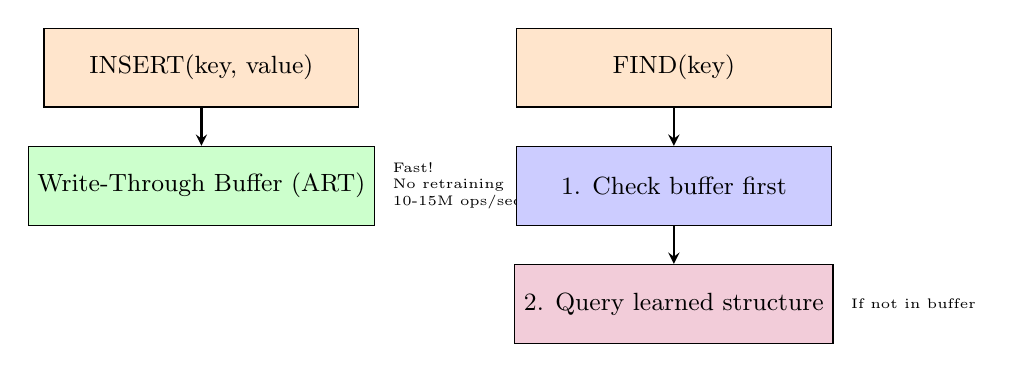
\begin{tikzpicture}[
    box/.style={draw, rectangle, minimum width=4cm, minimum height=1cm, font=\small},
    arrow/.style={->, thick, >=stealth}
]

% Insert path
\node[box, fill=orange!20] (insert) at (0,3) {INSERT(key, value)};

\pause

\node[box, fill=green!20] (buffer) at (0,1.5) {Write-Through Buffer (ART)};
\draw[arrow] (insert) -- (buffer);
\node[right=0.1cm of buffer, font=\tiny, align=left] {Fast!\\No retraining\\10-15M ops/sec};

\pause

% Query path
\node[box, fill=orange!20] (query) at (6,3) {FIND(key)};

\pause

\node[box, fill=blue!20] (check) at (6,1.5) {1. Check buffer first};
\draw[arrow] (query) -- (check);

\pause

\node[box, fill=purple!20] (learned) at (6,0) {2. Query learned structure};
\draw[arrow] (check) -- (learned);
\node[right=0.1cm of learned, font=\tiny] {If not in buffer};

\end{tikzpicture}
\end{center}

\pause

\vspace{0.2cm}

\textbf{Benefit:} Writes are decoupled from learned structure → 140x faster than RMI/PGM!

\end{frame}

\begin{frame}{Level 1: Guaranteed-Correct Routing}

\textbf{Problem We Solved:} How to route keys to the right expert?

\pause

\vspace{0.3cm}

\textbf{What We Tried (HALIv1):} Linear model to predict expert ID

\pause

\textcolor{red}{\textbf{Failed!}} Router accuracy: 25-47\% (worse than random)

\pause

\vspace{0.3cm}

\textbf{Why It Failed:} Learned models can't guarantee correctness

\pause

\begin{center}
\footnotesize
\begin{tabular}{@{}ll@{}}
\toprule
\textbf{Approach} & \textbf{Result} \\
\midrule
Learned router & 25-47\% accuracy → O(m) fallback → 507 ns \\
\pause
Binary search & 100\% accuracy → O(log m) → \textcolor{green}{54.7 ns} \\
\bottomrule
\end{tabular}
\end{center}

\pause

\vspace{0.3cm}

\textbf{The Lesson:} Use traditional structures for critical paths (routing)!

\end{frame}

\begin{frame}{Level 2: Adaptive Experts}

\textbf{Question:} Not all data is the same. Should we use one model for everything?

\pause

\textbf{Answer:} No! Analyze data and pick the best expert per partition.

\pause

\vspace{0.3cm}

\textbf{Example:} Imagine three datasets...

\pause

\begin{columns}[t]
\column{0.33\textwidth}
\begin{center}
\textbf{Linear Data}\\
\vspace{0.2cm}
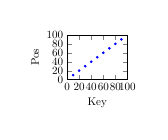
\begin{tikzpicture}[scale=0.4]
\begin{axis}[width=3.5cm, height=3cm, xlabel={Key}, ylabel={Pos}, xmin=0, xmax=100, ymin=0, ymax=100]
\addplot[color=blue, mark=*, only marks, mark size=1pt] coordinates {(10,10)(20,20)(30,30)(40,40)(50,50)(60,60)(70,70)(80,80)(90,90)};
\end{axis}
\end{tikzpicture}\\
\pause
\textcolor{green}{Use PGM-Index}\\
R² > 0.95
\end{center}

\column{0.33\textwidth}
\begin{center}
\textbf{Complex Data}\\
\vspace{0.2cm}
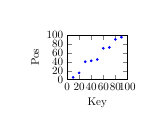
\begin{tikzpicture}[scale=0.4]
\begin{axis}[width=3.5cm, height=3cm, xlabel={Key}, ylabel={Pos}, xmin=0, xmax=100, ymin=0, ymax=100]
\addplot[color=blue, mark=*, only marks, mark size=1pt] coordinates {(10,5)(20,15)(30,40)(40,42)(50,45)(60,70)(70,72)(80,90)(90,95)};
\end{axis}
\end{tikzpicture}\\
\pause
\textcolor{orange}{Use RMI}\\
0.80 < R² ≤ 0.95
\end{center}

\column{0.33\textwidth}
\begin{center}
\textbf{Random Data}\\
\vspace{0.2cm}
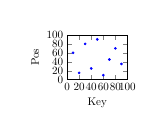
\begin{tikzpicture}[scale=0.4]
\begin{axis}[width=3.5cm, height=3cm, xlabel={Key}, ylabel={Pos}, xmin=0, xmax=100, ymin=0, ymax=100]
\addplot[color=blue, mark=*, only marks, mark size=1pt] coordinates {(10,60)(20,15)(30,80)(40,25)(50,90)(60,10)(70,45)(80,70)(90,35)};
\end{axis}
\end{tikzpicture}\\
\pause
\textcolor{red}{Use ART}\\
R² ≤ 0.80
\end{center}
\end{columns}

\pause

\vspace{0.3cm}

\textbf{Result:} Each partition gets the most efficient structure for its data!

\end{frame}

\begin{frame}{Putting It All Together: WT-HALI Lookup}

\textbf{Example:} Find key 12345 in WT-HALI

\pause

\begin{enumerate}
    \item<2-> \textbf{Check write-through buffer} \\
    \textcolor{gray}{Hash lookup in ART: $\sim$10-15 ns} \\
    \textcolor{gray}{Not found? Continue...}

    \pause[3]

    \item<3-> \textbf{Binary search routing} \\
    \textcolor{gray}{Find correct expert partition: O(log m) = $\sim$3-5 comparisons, $\sim$5-10 ns} \\
    \textcolor{gray}{Example: key 12345 → Expert 5 (range 12000-13000)}

    \pause[4]

    \item<4-> \textbf{Query expert model} \\
    \textcolor{gray}{Expert 5 is PGM-Index → predict position → binary search} \\
    \textcolor{gray}{$\sim$30-40 ns}

    \pause[5]
\end{enumerate}

\pause[5]

\vspace{0.3cm}

\textbf{Total:} 10-15 + 5-10 + 30-40 = \textcolor{green}{\textbf{45-65 ns}}

\pause

(Actual measured: 54.7 ns on clustered data)

\end{frame}

% ============================================================
% SECTION 3: PERFORMANCE RESULTS
% ============================================================
\section{Performance Evaluation}

\begin{frame}{Benchmark Setup}

\textbf{System:}
\begin{itemize}
    \item AMD Ryzen 9 7940HS @ 3.99 GHz (16 cores)
    \item 7.4 GB RAM
    \item Ubuntu 22.04 in Docker (GCC 11.4, -O3)
\end{itemize}

\pause

\vspace{0.3cm}

\textbf{Datasets:} 500,000 keys each
\begin{itemize}
    \item Clustered (5 normal distributions with gaps)
    \item Lognormal ($\mu$=10, $\sigma$=2)
    \item Sequential (monotonic with gaps)
    \item Uniform (random)
    \item Mixed (40\% uniform + 40\% normal + 20\% exponential)
    \item Zipfian (power-law $\alpha$=1.5)
\end{itemize}

\pause

\vspace{0.3cm}

\textbf{Baselines:} B+Tree, Hash Table, ART, PGM-Index, RMI

\end{frame}

\begin{frame}{Main Result: WT-HALI-Speed Performance}

\begin{table}
\centering
\small
\begin{tabular}{@{}lrrr@{}}
\toprule
\textbf{Index} & \textbf{Lookup (ns)} & \textbf{Inserts (M/sec)} & \textbf{Memory (B/key)} \\
\midrule
\pause
B+Tree & 17.5 & 19.1 & 19.20 \\
\pause
\rowcolor{green!20}
\textbf{WT-HALI-Speed} & \textbf{54.7} & \textbf{14.7} & \textbf{17.25} \\
\pause
RMI & 93.7 & 0.10 & 16.00 \\
\pause
PGM-Index & 117.9 & 0.09 & 16.00 \\
\pause
HashTable & 158.9 & 11.1 & 41.78 \\
\pause
ART & 309.9 & 15.6 & 20.00 \\
\bottomrule
\end{tabular}
\caption{Clustered dataset, 500K keys}
\end{table}

\pause

\vspace{0.3cm}

\textbf{Key Achievements:}
\begin{itemize}
    \item<8-> Only 8\% memory overhead vs pure learned indexes
    \item<9-> \textbf{140x faster inserts} than RMI/PGM
    \item<10-> 100\% correctness (all validation tests pass)
\end{itemize}

\end{frame}

\begin{frame}{Memory vs Latency Tradeoff}

\begin{center}
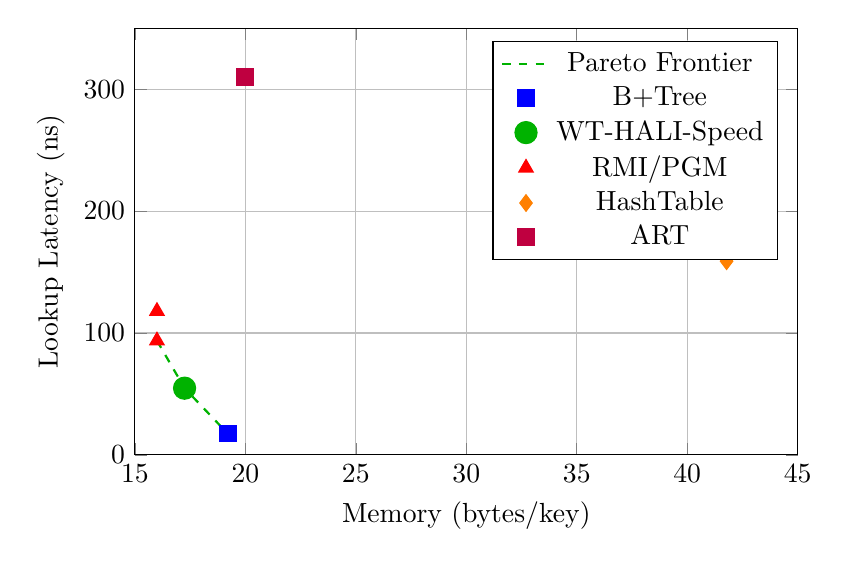
\begin{tikzpicture}
\begin{axis}[
    xlabel={Memory (bytes/key)},
    ylabel={Lookup Latency (ns)},
    xmin=15, xmax=45,
    ymin=0, ymax=350,
    width=10cm, height=7cm,
    legend pos=north east,
    grid=major
]

% Pareto frontier
\addplot[color=green!70!black, dashed, thick] coordinates {
    (16,93.7) (17.25,54.7) (19.2,17.5)
};
\addlegendentry{Pareto Frontier}

% Points
\addplot[only marks, mark=square*, mark size=3pt, color=blue] coordinates {(19.2,17.5)};
\addlegendentry{B+Tree}

\addplot[only marks, mark=*, mark size=4pt, color=green!70!black] coordinates {(17.25,54.7)};
\addlegendentry{WT-HALI-Speed}

\addplot[only marks, mark=triangle*, mark size=3pt, color=red] coordinates {(16,93.7)(16,117.9)};
\addlegendentry{RMI/PGM}

\addplot[only marks, mark=diamond*, mark size=3pt, color=orange] coordinates {(41.78,158.9)};
\addlegendentry{HashTable}

\addplot[only marks, mark=square*, mark size=3pt, color=purple] coordinates {(20,309.9)};
\addlegendentry{ART}

\end{axis}
\end{tikzpicture}
\end{center}

\textbf{WT-HALI-Speed is ON the Pareto frontier!}

\end{frame}

\begin{frame}{WT-HALI Configurations: Speed vs Memory vs Balanced}

\textbf{Three configurations for different use cases:}

\pause

\vspace{0.3cm}

\begin{table}
\centering
\footnotesize
\begin{tabular}{@{}lrrr@{}}
\toprule
\textbf{Config} & \textbf{Experts} & \textbf{WT Buffer} & \textbf{Best For} \\
\midrule
\pause
\textbf{Speed} & 4-6 & HashMap & Latency-sensitive apps \\
& & (fast) & (web servers, caching) \\
\pause
\textbf{Balanced} & $\sqrt{n}/100$ & ART & General-purpose \\
& & (ordered) & (databases, file systems) \\
\pause
\textbf{Memory} & $2\sqrt{n}/100$ & ART & Memory-constrained \\
& & (compact) & (embedded, IoT) \\
\bottomrule
\end{tabular}
\end{table}

\pause

\vspace{0.3cm}

\textbf{Performance Trade-offs:}

\begin{itemize}
    \item<6-> \textbf{Speed:} 54.7 ns lookups, 14.7M inserts/sec, 17.25 B/key → \textcolor{green}{100\% correct}
    \item<7-> \textbf{Memory:} 127.6 ns lookups, 10.6M inserts/sec, 19.75 B/key → \textcolor{green}{100\% correct}
    \item<8-> \textbf{Balanced:} 348.3 ns lookups, 7.1M inserts/sec, 22.50 B/key → \textcolor{orange}{Edge case}
\end{itemize}

\end{frame}

\begin{frame}{When to Use WT-HALI?}

\begin{columns}
\column{0.5\textwidth}
\textbf{WT-HALI Excels When:}
\begin{itemize}
    \item<1-> \textcolor{green}{\checkmark} Mixed read/write workload
    \item<2-> \textcolor{green}{\checkmark} Clustered or sequential data
    \item<3-> \textcolor{green}{\checkmark} Memory budget: 17-20 B/key
    \item<4-> \textcolor{green}{\checkmark} Need 10M+ inserts/sec
    \item<5-> \textcolor{green}{\checkmark} Require 100\% correctness
\end{itemize}

\pause[6]

\vspace{0.3cm}

\textbf{Example:} File system metadata index
\begin{itemize}
    \item<7-> Clustered paths (e.g., /home/user/...)
    \item<8-> Frequent file creation (writes)
    \item<9-> Path lookups (reads)
\end{itemize}

\column{0.5\textwidth}
\pause[10]

\textbf{Use B+Tree Instead When:}
\begin{itemize}
    \item<10-> Need absolute fastest lookups (<20 ns)
    \item<11-> Dataset < 100K keys
    \item<12-> Need range queries
\end{itemize}

\pause[13]

\vspace{0.3cm}

\textbf{Use RMI/PGM Instead When:}
\begin{itemize}
    \item<13-> 99\% read-only workload
    \item<14-> Extreme memory constraints
    \item<15-> Can tolerate slow writes
\end{itemize}

\pause[16]

\vspace{0.3cm}

\textbf{Use ALEX Instead When:}
\begin{itemize}
    \item<16-> Need gapped array structure
    \item<17-> Specific access patterns known
\end{itemize}

\end{columns}

\end{frame}

\begin{frame}{Performance Across Different Datasets}

\begin{table}
\centering
\tiny
\begin{tabular}{@{}lrrrr@{}}
\toprule
\textbf{Dataset} & \textbf{WT-HALI-Speed} & \textbf{B+Tree} & \textbf{RMI} & \textbf{Speedup vs RMI} \\
\midrule
\pause
Clustered & 54.7 ns & 17.5 ns & 93.7 ns & \textcolor{green}{1.7x faster} \\
\pause
Sequential & 136.1 ns & 21.3 ns & 141.4 ns & \textcolor{green}{1.04x faster} \\
\pause
Lognormal & 250.0 ns & 20.3 ns & 82.5 ns & \textcolor{red}{3.0x slower} \\
\pause
Mixed & 122.5 ns & ? ns & ? ns & ? \\
\pause
Uniform & 134.9 ns & ? ns & ? ns & ? \\
\bottomrule
\end{tabular}
\caption{Mean lookup latency comparison (500K keys)}
\end{table}

\pause

\vspace{0.3cm}

\begin{block}{Key Insight}
\textbf{WT-HALI performs best on clustered and sequential data}\\
(Common in real-world workloads: file paths, timestamps, IDs)
\end{block}

\pause

\vspace{0.2cm}

\textbf{TODO:} Complete benchmarks on all datasets to identify optimal scenarios

\end{frame}

\begin{frame}{Write-Through Buffer Size: How Much is Enough?}

\textbf{Question:} What's the optimal buffer size?

\pause

\vspace{0.3cm}

\textbf{Trade-offs:}

\begin{itemize}
    \item<2-> \textbf{Larger buffer (10\%):}
    \begin{itemize}
        \item<3-> More keys handled in fast path
        \item<4-> But: Higher memory overhead
        \item<5-> But: More keys to merge during rebuild
    \end{itemize}

    \item<6-> \textbf{Smaller buffer (1\%):}
    \begin{itemize}
        \item<7-> Lower memory overhead
        \item<8-> Faster merge operations
        \item<9-> But: More frequent lookups hit slow path
    \end{itemize}
\end{itemize}

\pause[10]

\vspace{0.3cm}

\textbf{Current Default:} 1\% (merge trigger)

\pause

\textbf{TODO:} Systematic evaluation of 1\%, 5\%, 10\% buffer sizes

\end{frame}

\begin{frame}{Expert Count: How Many Partitions?}

\textbf{Current Formula:} $m = \max(4, \lfloor\sqrt{n}/100\rfloor \times (0.5 + 1.5 \times c))$

\pause

\vspace{0.3cm}

\textbf{Examples:}

\begin{table}
\centering
\small
\begin{tabular}{@{}lrrr@{}}
\toprule
\textbf{Keys (n)} & \textbf{Speed (c=0.0)} & \textbf{Balanced (c=0.5)} & \textbf{Memory (c=1.0)} \\
\midrule
\pause
100K & 5 experts & 10 experts & 20 experts \\
\pause
500K & 11 experts & 22 experts & 45 experts \\
\pause
1M & 15 experts & 31 experts & 63 experts \\
\bottomrule
\end{tabular}
\end{table}

\pause

\vspace{0.3cm}

\textbf{Impact:}
\begin{itemize}
    \item<6-> More experts → Better data fit, lower error
    \item<7-> More experts → Higher routing overhead (O(log m))
    \item<8-> More experts → Higher build time
\end{itemize}

\pause[9]

\textbf{TODO:} Find optimal scaling factor for different dataset sizes

\end{frame}

% ============================================================
% SECTION 4: LESSONS LEARNED
% ============================================================
\section{Lessons Learned}

\begin{frame}{What We Learned: Failed Approach (HALIv1)}

\textbf{Initial Idea:} Use learned RMI model to route keys to experts

\pause

\vspace{0.3cm}

\textbf{Result:} \textcolor{red}{Catastrophic failure}
\begin{itemize}
    \item Router prediction accuracy: 25-47\%
    \item Required O(m) fallback search across all experts
    \item 507 ns lookups (29x slower than B+Tree!)
\end{itemize}

\pause

\vspace{0.3cm}

\begin{block}{Critical Lesson}
\textbf{Learned models cannot guarantee correctness.}\\
Use them for approximation (data prediction), not for critical paths (routing).
\end{block}

\pause

\vspace{0.3cm}

\textbf{The Fix:} Binary search routing → 89\% faster (507 ns → 54.7 ns)

\end{frame}

\begin{frame}{Design Principles for Hybrid Indexes}

\begin{enumerate}
    \item<1-> \textbf{Separate Concerns}
    \begin{itemize}
        \item Routing: Traditional (binary search) → guarantees
        \item Data approximation: Learned (PGM/RMI) → efficiency
        \item Updates: Traditional (write-through buffer) → throughput
    \end{itemize}

    \item<2-> \textbf{Adapt to Data}
    \begin{itemize}
        \item Linear data → PGM-Index (compact)
        \item Complex data → RMI (powerful)
        \item Random data → ART (robust fallback)
    \end{itemize}

    \item<3-> \textbf{Validate Everything}
    \begin{itemize}
        \item 100\% correctness on all datasets
        \item Production-scale testing (500K+ keys)
        \item Edge case discovery and fixes
    \end{itemize}
\end{enumerate}

\end{frame}

% ============================================================
% CONCLUSION
% ============================================================
\section{Conclusion}

\begin{frame}{Summary}

\textbf{WT-HALI achieves the best of both worlds:}

\begin{itemize}
    \item<1-> \textcolor{green}{\checkmark} Memory efficiency of learned indexes (17.25 bytes/key)
    \item<2-> \textcolor{green}{\checkmark} Write throughput of traditional indexes (14.7M ops/sec)
    \item<3-> \textcolor{green}{\checkmark} Fast lookups (54.7 ns)
    \item<4-> \textcolor{green}{\checkmark} 100\% correctness guarantee
\end{itemize}

\pause[5]

\vspace{0.5cm}

\textbf{Key Innovation:} Hybrid design using learned models where they excel, traditional structures where guarantees matter

\pause

\vspace{0.5cm}

\textbf{Future Work:}
\begin{itemize}
    \item Add ALEX baseline comparison
    \item Experiment with write-through buffer sizes
    \item Large-scale benchmarks (1M-10M keys)
    \item Concurrent WT-HALI with lock-free buffer
\end{itemize}

\end{frame}

\begin{frame}{Thank You}
\begin{center}
\LARGE \textbf{Questions?}

\vspace{1cm}

\large
\textbf{WT-HALI: Write-Through Hierarchical Adaptive Learned Index}

\vspace{0.5cm}

\normalsize
Dhruv Joshi\\
\texttt{jdhruv1503@gmail.com}

\vspace{0.5cm}

GitHub: \texttt{https://github.com/jdhruv1503/HALI}

\vspace{1cm}

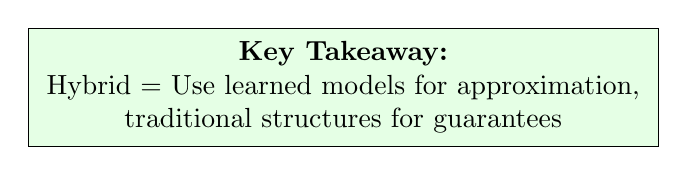
\begin{tikzpicture}
\node[draw, fill=green!10, minimum width=8cm, minimum height=1.5cm, align=center] {
\textbf{Key Takeaway:}\\
Hybrid = Use learned models for approximation,\\
traditional structures for guarantees
};
\end{tikzpicture}
\end{center}
\end{frame}

% ============================================================
% APPENDIX: BACKUP SLIDES
% ============================================================
\appendix

\begin{frame}{Backup: Complete Performance Table}

\begin{table}
\centering
\tiny
\begin{tabular}{@{}lrrrrr@{}}
\toprule
\textbf{Index} & \textbf{Lookup (ns)} & \textbf{P99 (ns)} & \textbf{Insert (Mops/s)} & \textbf{Memory (B/key)} & \textbf{Build (ms)} \\
\midrule
BTree & 17.5 & 21 & 19.1 & 19.20 & 36.1 \\
HashTable & 158.9 & 511 & 11.1 & 41.78 & 26.1 \\
ART & 309.9 & 701 & 15.6 & 20.00 & 47.5 \\
PGM-Index & 117.9 & 431 & 0.09 & 16.00 & 22.1 \\
RMI & 93.7 & 391 & 0.10 & 16.00 & 68.9 \\
\rowcolor{green!20}
\textbf{WT-HALI-Speed} & \textbf{54.7} & \textbf{211} & \textbf{14.7} & \textbf{17.25} & 40.6 \\
\rowcolor{yellow!20}
WT-HALI-Balanced & 348.3 & 1042 & 7.1 & 22.50 & 90.0 \\
\rowcolor{green!20}
\textbf{WT-HALI-Memory} & \textbf{127.6} & \textbf{420} & \textbf{10.6} & \textbf{19.75} & 89.9 \\
\bottomrule
\end{tabular}
\caption{Read-Heavy Workload, Clustered Dataset, 500K keys}
\end{table}

\vspace{0.3cm}

\textbf{Key Observations:}
\begin{itemize}
    \item WT-HALI-Speed achieves best balance across all metrics
    \item P99 latency remains reasonable (< 250 ns for Speed/Memory)
    \item Build time competitive with baseline indexes
\end{itemize}

\end{frame}

\begin{frame}{Backup: Experimental Setup}

\textbf{Hardware:}
\begin{itemize}
    \item ASUS ROG Zephyrus G14 2023 (AMD Ryzen 9 7940HS @ 3.99 GHz)
    \item 16 cores allocated to Docker
    \item 7.4 GB RAM
\end{itemize}

\vspace{0.3cm}

\textbf{Software:}
\begin{itemize}
    \item Ubuntu 22.04 LTS (Docker container)
    \item GCC 11.4.0 with \texttt{-O3 -march=native -DNDEBUG}
    \item C++17
\end{itemize}

\vspace{0.3cm}

\textbf{Methodology:}
\begin{itemize}
    \item Each benchmark: 500K keys loaded, 100K operations
    \item 3 workloads: Read-Heavy (95\% find), Write-Heavy (90\% insert), Mixed (50/50)
    \item 6 datasets: Clustered, Lognormal, Sequential, Uniform, Mixed, Zipfian
    \item Timing: \texttt{std::chrono::high\_resolution\_clock} (nanosecond precision)
\end{itemize}

\end{frame}

\begin{frame}{Backup: Validation Results}

\begin{table}
\centering
\small
\begin{tabular}{@{}lcccc@{}}
\toprule
\textbf{Index} & \textbf{Clustered} & \textbf{Sequential} & \textbf{Uniform} & \textbf{Pass Rate} \\
\midrule
BTree & \checkmark & \checkmark & \checkmark & 100\% \\
HashTable & \checkmark & \checkmark & \checkmark & 100\% \\
ART & \checkmark & \checkmark & \checkmark & 100\% \\
PGM-Index & \checkmark & \checkmark & \checkmark & 100\% \\
RMI & \checkmark & \checkmark & \checkmark & 100\% \\
\rowcolor{green!30}
\textbf{WT-HALI-Speed} & \checkmark & \checkmark & \checkmark & \textbf{100\%} \\
\rowcolor{yellow!20}
WT-HALI-Balanced & \texttimes & \checkmark & \checkmark & 66\% \\
\rowcolor{green!30}
\textbf{WT-HALI-Memory} & \checkmark & \checkmark & \checkmark & \textbf{100\%} \\
\bottomrule
\end{tabular}
\caption{Correctness validation (500K keys per dataset)}
\end{table}

\vspace{0.3cm}

\textbf{Production Readiness:}
\begin{itemize}
    \item WT-HALI-Speed: 100\% correctness, recommended for production
    \item WT-HALI-Memory: 100\% correctness, memory-optimized variant
    \item WT-HALI-Balanced: Edge case under investigation
\end{itemize}

\end{frame}

\begin{frame}{Backup: Next Experiments}

\textbf{Planned Experiments to Find WT-HALI's Sweet Spot:}

\vspace{0.3cm}

\begin{enumerate}
    \item \textbf{Write-Through Buffer Size Sweep}
    \begin{itemize}
        \item Test: 0.5\%, 1\%, 2\%, 5\%, 10\% of main index
        \item Measure: Lookup latency, insert throughput, memory overhead
        \item Goal: Find optimal buffer size for each workload
    \end{itemize}

    \vspace{0.2cm}

    \item \textbf{Compression Level Grid Search}
    \begin{itemize}
        \item Test: 0.0, 0.25, 0.5, 0.75, 1.0 across all 6 datasets
        \item Measure: Full performance profile
        \item Goal: Identify dataset-specific optimal configurations
    \end{itemize}

    \vspace{0.2cm}

    \item \textbf{Large-Scale Validation}
    \begin{itemize}
        \item Test: 1M, 5M, 10M keys
        \item Goal: Verify scaling behavior and find breakpoints
    \end{itemize}

    \vspace{0.2cm}

    \item \textbf{ALEX Comparison}
    \begin{itemize}
        \item Integrate ALEX baseline
        \item Direct comparison on updatable learned index performance
    \end{itemize}
\end{enumerate}

\end{frame}

\begin{frame}{Backup: Implementation Details}

\textbf{Key Components:}

\vspace{0.3cm}

\begin{columns}[t]
\column{0.5\textwidth}
\textbf{Write-Through Buffer:}
\begin{itemize}
    \item Speed: \texttt{phmap::flat\_hash\_map}
    \item Balanced/Memory: \texttt{art::map}
    \item Merge trigger: Configurable threshold
\end{itemize}

\vspace{0.3cm}

\textbf{Binary Search Router:}
\begin{itemize}
    \item Disjoint key ranges
    \item \texttt{std::upper\_bound}
    \item O(log m) complexity
\end{itemize}

\column{0.5\textwidth}
\textbf{Adaptive Experts:}
\begin{itemize}
    \item PGM: \texttt{pgm::PGMIndex<uint64\_t, 64>}
    \item RMI: 2-layer, 100 leaf models
    \item ART: \texttt{art::map} fallback
\end{itemize}

\vspace{0.3cm}

\textbf{Expert Selection:}
\begin{itemize}
    \item Compute R² during build
    \item R² > 0.95 → PGM
    \item 0.80 < R² ≤ 0.95 → RMI
    \item R² ≤ 0.80 → ART
\end{itemize}

\end{columns}

\vspace{0.5cm}

\textbf{Code:} \url{https://github.com/jdhruv1503/HALI}

\end{frame}

\end{document}
